\chapter{Data}

\section{Data Acquisition}

This research project utilises the most recent open access spectral data from the GALAH survey. At the time of writing, the GALAH survey is in its third data release (GALAH DR3). GALAH DR3 comprises 678,423 spectra for 588,571 stars, of which approximately 80\% of these stars are within a radius of 2 kpc \cite{buder2021galah+}. Of the 588,571 stars, continuum normalised spectra of 588,343 have been provided.The GALAH DR3 (hereafter DR3) is accessible via the \href{https://www.galah-survey.org/}{survey website} and \href{https://datacentral.org.au/}{AAO Data Central}. DR3 provides continuum normalised spectra and errors for a majority of spectra and candidates. In the case of problematic reductions, for candidates where this is not possible, object IDs and flags have been provided. This study avoids using these problematic spectra.

The data is organised as individual \texttt{.fits} format files. Each file contains an object ID prefix (known as an "\texttt{sobject\_id}") followed the last digit in the filename which serves as the camera number suffix. Thus, the file \texttt{1705090057010093.fits} is a data file for an object with \texttt{sobject\_id=170509005701009} and contains spectral data from camera 3 (or the red camera). The blue, green and infra red cameras are denoted by the suffix 1,2 and 4 respectively.
The red camera of the HERMES spectrograph is the spectral channel with the range 6478\r{A} - 6737\r{A}\cite{sheinis2014first}. This range is of particular interest to this research as the characteristic H$\alpha$ line appears within this range. These individual files totalling 385 GB were downloaded to a Macquarie University file server and served as the data source for all research and analytical work presented in this thesis.

\begin{figure}[h]
\centering
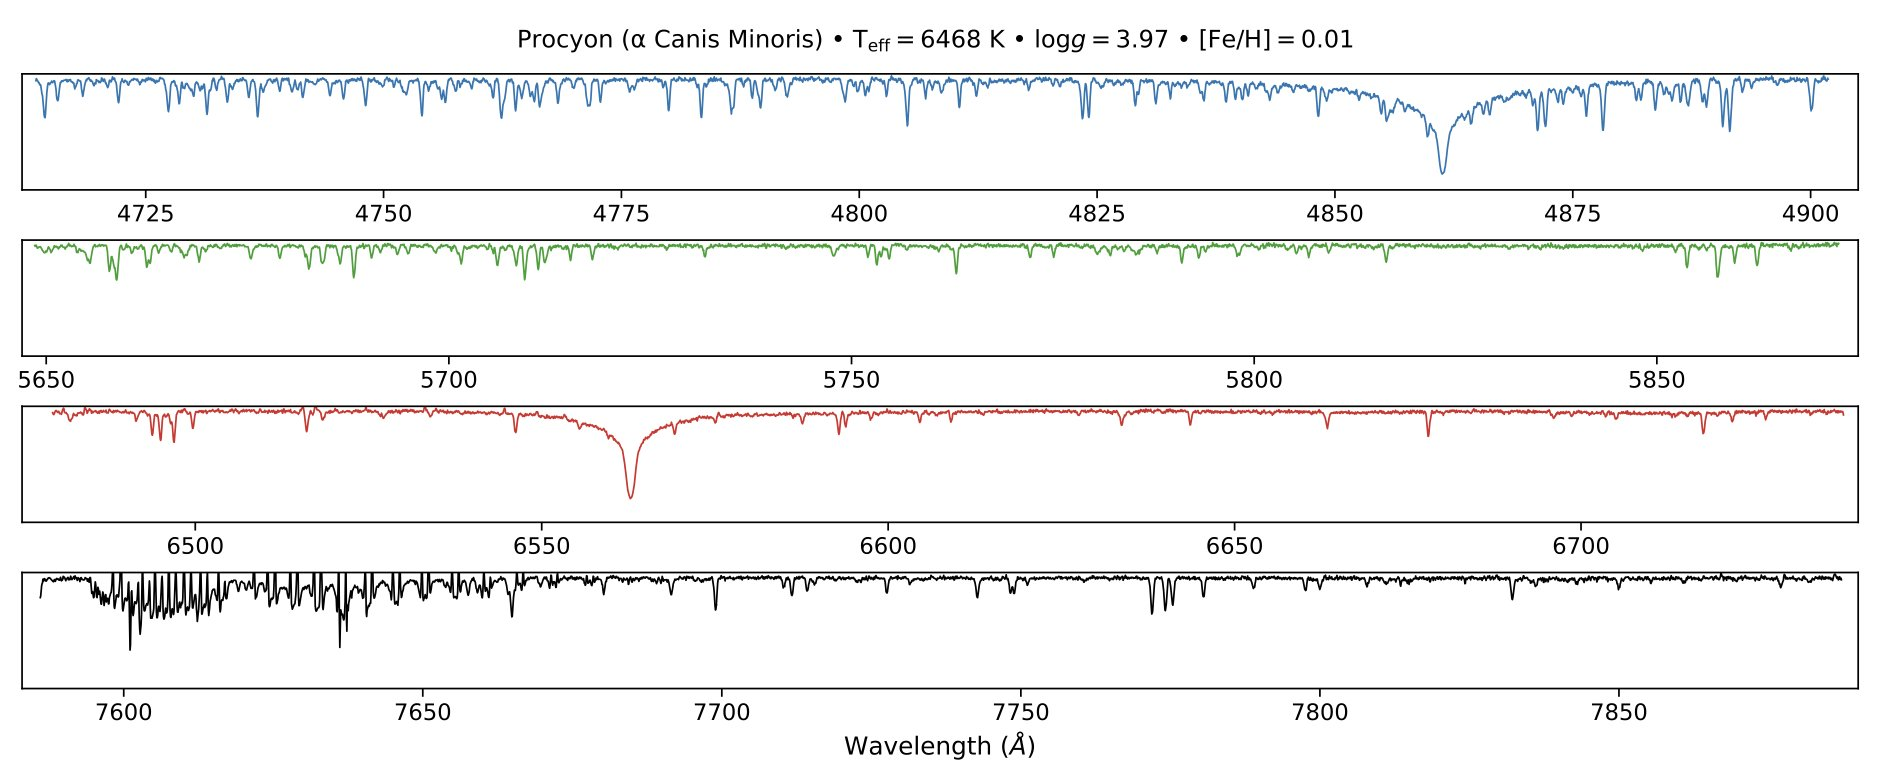
\includegraphics[scale=.25]{figures/galah cameras.jpeg}
\caption{Normalised DR3 spectral data for the star $\alpha$ Canis Minoris.}
\end{figure}

Given that spectral features are recorded across four cameras, the feature space of this data is significant. As an illustrative example, consider the red camera only. The feature space calculation is as follows.
\[\lambda_{min} = 6478\]
\[\lambda_{max} = 6737\]
\[\Delta\lambda \approx 0.06\]
Where $\Delta\lambda$ is the wavelength separation equivalent of the sampling rate of the wavelength grid of the individual spectrum. Thus the size of the wavelength grid is given by, \[N_{\lambda} = (\lambda_{max}-\lambda_{min})/\Delta\lambda \approx (6737-6478)/0.06 \approx 4317\]
This will be equal to the number of features in the red camera of a given spectrum, \[N_{f} \approx 4317\]
Thus the total number of features for the red camera across DR3 is, \[N_{T} \approx 4317\times678,423 \approx \num[round-precision=2,round-mode=figures,
     scientific-notation=true]{2928752091}\]

\begin{figure}[t]
\centering
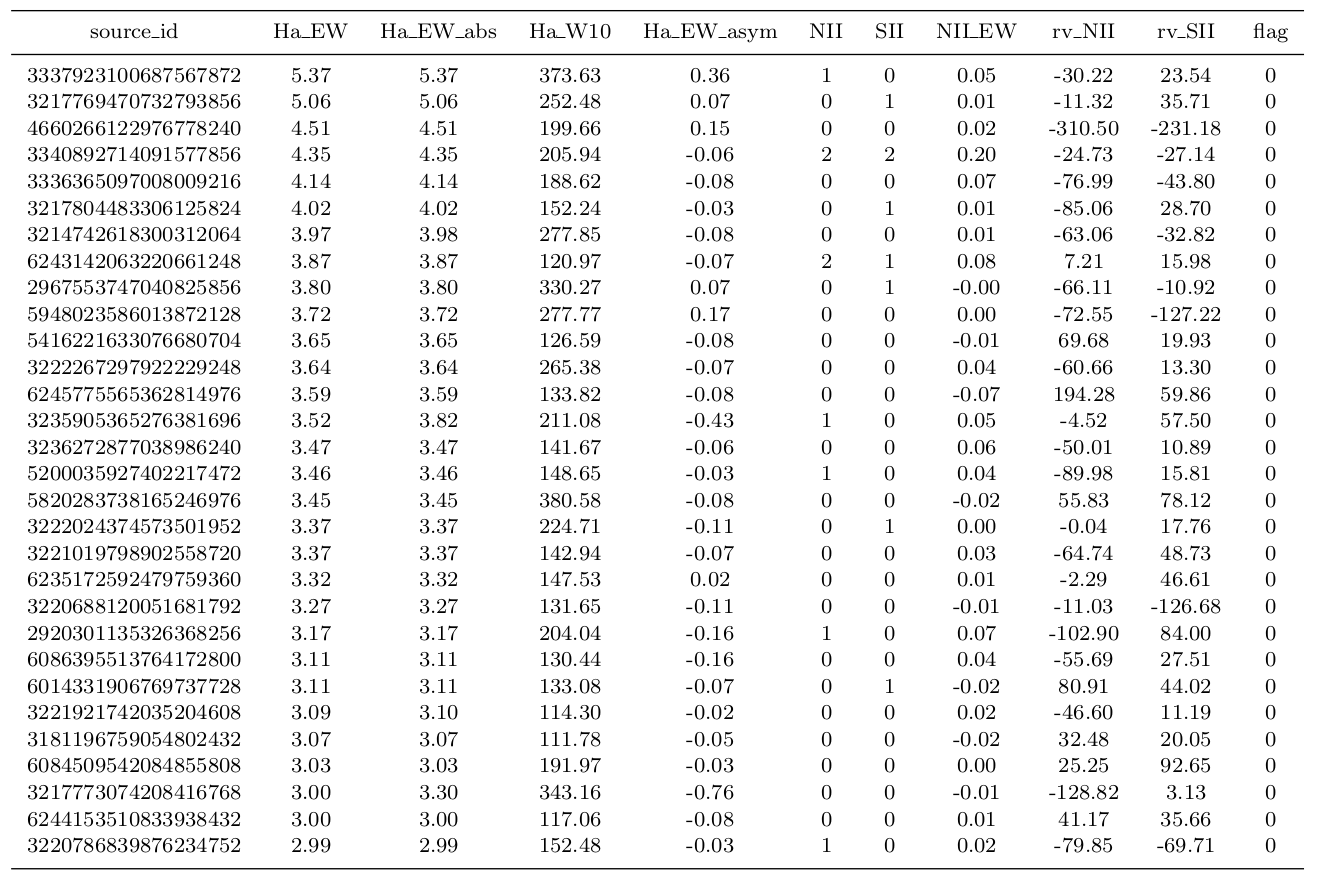
\includegraphics[scale=.35]{figures/cotartable.png}
\caption{The 30 strongest emitters. Reproduced from Čotar et al. (2021)\cite{vcotar2021galah}}
\end{figure}
This calculation naively implies the existence of a billion scale feature space, and consequently a potentially billion dimensional vector space. Thus the data analysis and machine learning strategy will have to be chosen carefully. If care is not taken during feature engineering and pre-processing steps, the volume of data will lend itself to what is colloquially referred to as the "curse of dimensionality". The curse of dimensionality implies an extraordinarily rapid growth in the difficulty of problems as the number of variables (or the dimension) increases \cite{kuo2005lifting}.

This research will also utilise a recently published dataset of H$\alpha$ candidates in DR3. Published in 2020, Čotar et al. used DR3\cite{de2015galah}, the K2-HERMES survey\cite{wittenmyer2018k2} and the TESS-HERMES survey\cite{sharma2018tess} to derive a catalogue of potential H$\alpha$ emission stars using an automated supervised machine learning pipeline. Combining data from three surveys, this study used 669,845 continuum normalised stellar spectra as a data input source and included a small fraction of repeated observations. The study identified 10,364 candidate spectra with varying degree of H$\alpha$ emission components. Summarised information of these candidates, their object IDs, including DR3 \texttt{sobject\_ids} were released via \href{https://cdsweb.u-strasbg.fr/}{CDS} as open access data. This data was presented as a single \texttt{.fits} format file. No spectral information was provided with this dataset. The 30 strongest emitters from this study are presented in Figure 2.2 above. The benefit of using this dataset over the entire DR3 is that there will be a higher chance of identifying P Cygni and inverse P Cygni spectra given essentially the pre-selection of H$\alpha$ candidates by Čotar et al. P Cygni and inverse P Cygni spectra are a subset of H$\alpha$ emission spectra. However, one limitation of using this dataset exclusively is that the potential number of identifable P Cygni stars will be limited by the number of H$\alpha$ candidates identified by Čotar et al. only. Presumably this dataset does contain all H$\alpha$ candidates in DR3 but it does not guarantee it. 

\section{Spectra as Time Series}

The normalised flux recorded by each camera as a function of wavelength can be considered to have behaviour similar to a "time series". While a monotonically increasing time axis is not included in the data, the monotonically increasing wavelength grid can serve as an analogue to the time axis. Thus a plot of normalised flux against wavelength represents the variation of a flux against wavelength similar to the variation of a time dependent quantity against the time axis.

As it shall be demonstrated in subsequent chapters, this is an unconventional yet incredibly powerful approach to spectral analysis. Precedent for this approach can be found in related fields such as chemistry and nuclear magnetic resonance (NMR) spectroscopy where NMR spectra are subjected to signal processing techniques originally developed for time series analysis \cite{nielsen2019practical}. 

\section{Data Resampling}

In order to isolate the red camera data ("camera 3"), the following process was carried out. All filenames of the DR3 \texttt{.fits} format files were read into an array. Files with the suffix "3" were then selected. Additionally the number "3" was stripped from this sub array of file names to generate a list of \texttt{sobject\_id} values. This significantly simplifies data querying and reading operations as all standard query and file read operations rely on only \texttt{sobject\_id} and not the file name that includes the \texttt{sobject\_id} and camera suffix. 

The added advantage of this approach is that it automatically excludes \texttt{sobject\_id} values for which red camera data does not exist. A list of such \texttt{sobject\_id} values is published on the GALAH survey website. However this study did not require the use of this list as the procedure above infers these \texttt{sobject\_id} values directly from the \texttt{.fits} filenames. This process results in a collection of 588,344 \texttt{sobject\_id} values. This is lower than the 588,571 total number of stars recorded by DR3. The difference is attributed to those stars for which the normalised red camera data doesn't exist. 

\begin{figure}[h]
\centering
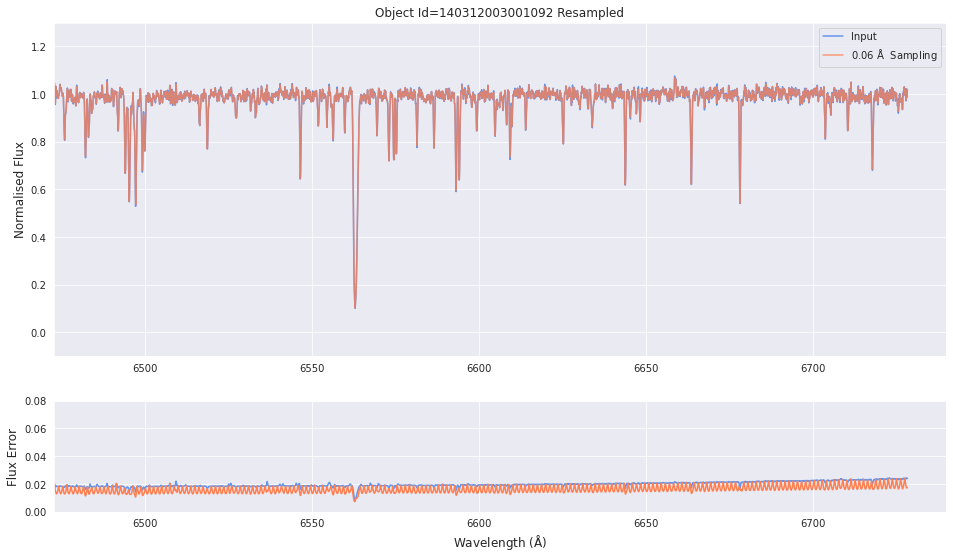
\includegraphics[scale=.40]{figures/resampling example.png}
\caption{Resampling a DR3 spectrum and it's error spectrum to a common wavelength grid.}
\end{figure}

The sampling rate for each observed spectrum can vary. For the red camera, this rate is equivalent to a wavelength separation of $\Delta\lambda$ $\approx$ 0.06 \r{A}\cite{vcotar2021galah}. The sampling rate of each spectrum from the red camera was found to vary around this value at the third decimal. For subsequent analysis each spectrum is required to be a vector of fixed size. A collection of spectra i.e. the total dataset that will be subjected to analysis must consist of a uniform set of these vectors. The advantage of this approach is that spectral features, particularly morphological features can be compared against each other more effectively. Thus the spectra under consideration were interpolated to a common wavelength grid with a sampling rate equivalent to 0.06 \r{A}. This rate was chosen so that oversampling and under-sampling would be significantly minimized. This rate is accurate to the sampling rate of each spectrum generated by the red camera to the second decimal place. 

Data resampling or interpolation in the context of spectral data is a common operation in astronomy. This work uses the \texttt{spectres} Python package \cite{carnall2017spectres} to efficiently sample all red camera spectra to the following common wavelength grid.

\[\lambda_{min} = 6472.5\]
\[\lambda_{max} = 6740\]
\[\Delta\lambda = 0.06\]

This grid was chosen based on the range of spectral values and wavelength separation observed in the raw data. Normalised spectra and their errors from the red camera were subjected to this interpolation scheme. The authors of DR3 have set the continuum value for the normalised spectra at 1. Thus, spectra for which flux values were not recorded at the tail and top end of the interpolated grid, were padded with the value 1 in order to maintain the uniformity of the common wavelength grid. Resampling is computationally intensive and thus this process was offloaded to a university science server. The resultant data and interpolated errors were saved as HDF5 files using the \texttt{.h5} file format in a single array for convenience. 

\section{Region Selection}

The total number of spectral features for the red camera is $\approx$ \num[round-precision=2,round-mode=figures, scientific-notation=true]{2928752091}. P Cygni and inverse P Cygni stars show characteristic emission and absorption profiles near the H$\alpha$ line. This observation can be exploited to significantly reduce the size of the feature space. 
The region of interest around H$\alpha$ was selected to be 6561\r{A} - 6565\r{A} \cite{traven2017galah}. Repeating the feature space calculation above it can be noted that this region is sufficiently narrow enough to reduce the feature space by a hundredfold to $\approx$ \num[round-precision=2,round-mode=figures, scientific-notation=true]{45228200} while simultaneously ensuring that it can encapsulate emission features for P Cygni and inverse P Cygni spectra. In code, this selection was implemented as a binary spectral mask which extracts the flux values for the relevant wavelength range while masking flux values outside it. A masked version of the resampled data was stored in a separate \texttt{.h5} file.

